\documentclass[12pt,french]{article}
\usepackage[utf8]{inputenc}
\usepackage[T1]{fontenc}
\usepackage{mathtools}
\usepackage[scale=0.8]{geometry}

\usepackage{amsmath}
\usepackage{graphicx}
\graphicspath{{images/}}
\usepackage{parskip}
\usepackage{fancyhdr}
\usepackage{vmargin}
\usepackage{hyperref}

\setmarginsrb{3 cm}{2.5 cm}{3 cm}{2.5 cm}{1 cm}{1.5 cm}{1 cm}{1.5 cm}

\title{Tutoriel d'introduction à angular.schematics}								
\author{Louiza AOUCHETA}								
\date{\today}											

\makeatletter
\let\thetitle\@title
\let\theauthor\@author
\let\thedate\@date
\makeatother

\pagestyle{fancy}
\fancyhf{}
\rhead{\theauthor}
\lhead{\thetitle}
\cfoot{\thepage}


\begin{document}


%%%%%%%%%%%%%%%%%%%%%%%%%%%%%%%%%%%%%%%%%%%%%%%%%%%%%%%%%%%%%%%%%%%%%%%%%%%%%%%%%%%%%%%%%

\begin{titlepage}
\centering 
\includegraphics[scale=0.25]{../../../../Images/image.jpg} \\
    \vspace*{0.5 cm}
    \textsc{\LARGE Master 2: EID2}\\[2.0 cm]	
	\textsc{\large Langage et Environnement Evolues}\\[0.5 cm]				% Course Name
	\rule{\linewidth}{0.2 mm} \\[0.4 cm]
	{ \huge \bfseries \thetitle}\\
	\rule{\linewidth}{0.2 mm} \\[1.5 cm]
	
	\begin{minipage}{0.4\textwidth}
		\begin{flushleft} \large
			\emph{Réalisé par:}\\
			\theauthor
			\end{flushleft}
			\end{minipage}~
			\begin{minipage}{0.4\textwidth}
			\begin{flushright} \large
			\emph{Encadré par:} \\
			M. P.BOUDES									% Your Student Number
		\end{flushright}
	\end{minipage}\\[2 cm]
	
	{\large \thedate}\\[2 cm]
 
	\vfill
	
\end{titlepage}

		\qquad\qquad\qquad\large{\textbf{Tutoriel d’introduction à Angular.Schematics.}}\newline
	
	Avant de commencer le tutoriel sur l'utilisation de \textbf{angular.schematics}, on va débuter par un bref aperçu sur ce qu'est \textbf{schematics} (schémas) et pourquoi ils sont utiliser.\newline
	
	\textbf{I.Présentation de angular schematics}\newline
	
	Schematics en français schémas est un outil de workflow pour le Web moderne.\newline
	Dans Angular on entend souvent parler de Schematics et Collection.\smallbreak
	schematics - est une "recette" qui peut être exécutée en utilisant ng generate <schematic-name>pour générer et ajuster des fichiers de projet\smallbreak
	collection - (qui est une collection de schémas c'est à dire une liste de schémas) est un package (package npm) qui contient au moins un schéma.\newline
	
	Si on utilise Angular CLI, nous pouvons exécuter beaucoup de schémas par défaut car ils sont inclus dans la @schematics/angular collection. Cela permet de générer des éléments tels que des composants ou des services.\newline
	
	Nous pouvons également installer une collection supplémentaire à partir de \textbf{npm} et exécuter ses schémas en transmettant un \textbf{\--\--collection} comme indicateur supplémentaire à ng generate tel que si on fait ng generate <schematic-name> \--\--collection <collection-name>.\newline
	
	En général, les schémas permettent de:\smallbreak
		\quad-Ajouter des bibliothèques à un projet angular,\smallbreak
		\quad-Mettre à jour des bibliothèques dans un projet angular\smallbreak
		\quad-Générer du code.\smallbreak
		\quad-Créer un nouveau composant ou mettre à jour du code pour corriger des modifications 		importantes d'une dépendance\smallbreak
		\quad-Ajouter une nouvelle option de configuration ou une nouvelle structure à un projet existant.\newline
		
	 Exemples d'avantages pour créer une collection de schémas:\smallbreak
	\quad-Génération de modèles d'interface utilisateur couramment utilisés dans une application.\smallbreak
	\quad-Génération de composants spécifiques à l'organisation à l'aide de modèles ou de 	présentations prédéfinis.\smallbreak
	\quad-Mise en application de l'architecture organisationnelle.
\newline

	\textbf{II. Création d'un premier schéma}\newline
	
	Avant de créer un schéma angular il est nécessaire de s'assurer que Node 6.9 ou une version supérieur est bien installé sur la machine sur lequel le travail doit être effectué. 
	Ensuite, installez Schematics via une de commande:
\newline
	
	\qquad sudo npm install -g @angular-devkit / schematics-cli \newline
	
	Cela installera un exécutable de schematics.\newline
	\\
	\includegraphics[scale=0.65]{../projet/install_schematics.png} 
	
	Maintenant que nous avons installé l'outil via une ligne de commande, nous avons accès à cet exécutable, cependant, nous avons la possibilité de créer un nouveau projet de schémas vierge à l'aide de Schematics CLI:\newline
	
	\qquad louiza@louiza-Satellite-C660:$\sim$node\_modules\$ schematics blank \--\--name=first-try\newline
	
	En exécutant cette ligne de commande nous observons que tous les fichiers liés au schéma sont créés\newline
	
	\begin{tabular}{l}
		\qquad CREATE /first-try/README.md (639 bytes)\\
		\qquad CREATE /first-try/package.json (536 bytes)\\
		\qquad CREATE /first-try/tsconfig.json (656 bytes)\\
		\qquad CREATE /first-try/.gitignore (191 bytes)\\
		\qquad CREATE /first-try/.npmignore (64 bytes)\\
		\qquad CREATE /first-try/src/collection.json (222 bytes)\\
		\qquad CREATE /first-try/src/first-try/index.ts (315 bytes)\\
		\qquad CREATE /first-try/src/first-try/index\_spec.ts (468 bytes)
	\end{tabular}\break

	 Une fois le projet créé nous pouvons l’ouvrir dans un environnement de travail qui prend en charge angular tel que WebStorm et nous allons voir qu’un schéma dispose réellement de 4 principaux fichiers .\newline

	-package.json : contient le nom du projet, sa version, sa description ainsi que certaines dépendances pour déboguer et tester des scripts et la propriété la plus importante est schematics qui dispose d’un chemin vers le fichier collection.son\smallbreak
	-collection.json: contient la définition du schéma\smallbreak
	-index.ts: représente le code schematics réel\smallbreak
	-ts.config : représente la configuration du compilateur TypeScript\newline
	
	A l'intérieur du dossier \textbf{src} nous allons trouver le fichier \textbf{collection.json}, en ouvrant ce fichier nous observons que le bout de code suivant est généré automatiquement\newline
	
	\begin{tabular}{ll}
		\{&\\
		&"\$schema":\\ &"../node\_modules/@angular-devkit/schematics/collection-schema.json",\\
		&"schematics": \{\\
		&\quad"first-try": \{
\\
		&\qquad"description": "A blank schematic.",
\\
		&\qquad"factory": "./first-try/index\#firstTry"\\
		&\quad \}
\\
		& \}
\\
		\}
	\end{tabular}\break

	La clé importante est "schematics" , qui décrit les schémas inclus dans cette collection. 
	Dans notre exemple, nous décrivons un schéma: first-try , il a une description simple avec un champ factory.\\
	Le champ factory est une chaîne de caractères (string) qui spécifie l'emplacement du fichier du point d'entrée de notre schéma, suivi d'un symbole de hachage, suivi de la fonction qui sera appelée. Dans  ce cas, nous invoquerons la fonction firstTry() dans le fichier first-try / index.ts  qui fait référence à une chaîne de caractères pour pointer sur une fonction JavaScript. Il représente le RuleFactory .\newline 
	
	Une Rule (règle) est une fonction qui prend un Tree (arbre) et retourne un autre Tree . Les règles sont au cœur des schémas; ce sont eux qui apportent des modifications aux projets, appellent des outils externes et implémentent une logique. Comme son nom l'indique une RuleFactory est une fonction qui crée une règle dite Rule.\\
	L'arbre Tree est une structure de données qui contient une base (un ensemble de fichiers déjà existants) et une zone de stockage intermédiaire (liste des modifications à appliquer à la base).\\
	Lorsque des modifications sont apportées, il n'y a pas de changement réel de la base, mais nous ajoutons ces modifications à la zone intermédiaire.\newline
	
	Le Tree est utilisé par angular CLI et représente le projet sur le lecteur jusqu'au premier schéma appelé, mais les schémas composés peuvent recevoir n’importe quel Tree.\newline
	
	Voici le RuleFactory vierge créé jusqu'à présent dans index.ts\newline
	
	import \{ Rule, SchematicContext, Tree \} from '@angular-devkit/schematics';\newline
	
	\textit{// You don't have to export the function as default. You can also have more than one rule factory}\newline
	\textit{// per file.}\newline	
	\begin{tabular}{l}
		export function \textit{firstTry}(\_options: any): Rule \{\\
		\quad return (tree: Tree, \_context: SchematicContext) => \{\\
		\qquad return tree;\\
		\quad\};\\
		\}\\
	\end{tabular}\break

	La fonction firstTry prend en argument un ensembles d'options et retourne une Rule qui prend un Tree et le retourne inchangé.\newline
	
	L'argument \_options est un objet qui peut être considéré comme un input. Dans la CLI, il s'agit des arguments de ligne de commande que l'utilisateur a transmis. Du point de vue d'un autre schéma, ce sont les options qui ont été transmises par ce schéma.\newline
	
	Dans la plupart des cas, il s’agit souvent d’un objet quelconque et peut être saisi par any . Il peut également être validé avec un schéma JSON pour assurer que les entrées ont les types et valeurs par défaut appropriés.\newline
	
	Il est aussi possible de créer un fichier à la racine du Tree du schéma de la RuleFactory nommé d'après \_options.name "hello" et qui contient la chaîne de caractère "world". \newline
	
	import \{ Rule, SchematicContext, Tree \} from '@angular-devkit/schematics';\newline
	
	\textit{// You don't have to export the function as default. You can also have more than one rule factory}\\
	\textit{// per file}.
\newline
	
		\begin{tabular}{l}
		export function \textit{firstTry}(\_options: any): Rule \{ \\
			\quad return (tree: Tree, \_context: SchematicContext) => \{ \\
				\qquad tree.create ('hello',"Hello World")\\
				\qquad return tree;\\
			\quad\};
\\
		\}
	\end{tabular}\break\\
	\\
	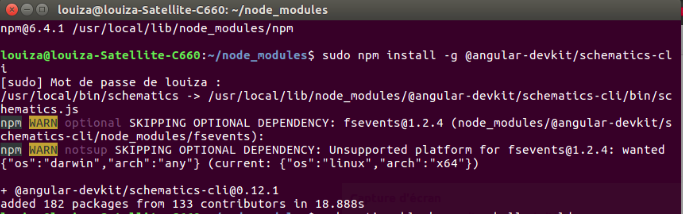
\includegraphics[scale=0.65]{../projet/1.png} 

	Pour résumer, un Tree contient les fichiers sur lesquels les schémas doivent être appliqués. Il contient une liste de fichiers et contient des métadonnées associées aux modifications souhaitées. Dans notre cas, la seule modification apportée consiste à créer un nouveau fichier et sont considérés comme une collection de fichiers et de modifications.\newline
	Par défaut, angular CLI transmet la racine du projet angular en tant que Tree , mais tout schéma peut être transmis à un Tree différent des autres. De plus il existe quatre méthodes qui créent directement un changement dans un Tree et qui sont : create , delete , rename et overwrite.\newline
	
	\textbf{III. Exécution d'un  schéma angular}\newline
	
	Pour exécuter notre exemple, il est impératif d'utiliser l'outil de ligne de commande "schematics" avec le chemin d'accès au répertoire de notre projet \\schématique en tant que "collection".\newline  
	
	louiza@louiza-Satellite-C660:$\sim$/node\_modules\$ npm run build \newline
	
	\begin{tabular}{l}
		\# ... attend la fin de la construction et on obtient\\ 
		\qquad > first-try@0.0.0 build /home/louiza/node\_modules/first-try\\
		\qquad > tsc -p tsconfig.json
\\
		Process finished with exit code 0
	\end{tabular}\break
	
	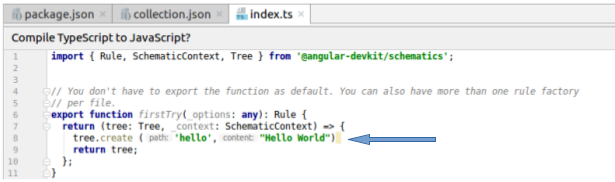
\includegraphics[scale=0.75]{../projet/2.png} 

	Cette dernière ligne veut dire que l’exécution ne retourne aucune erreur\newline
	
	\begin{tabular}{l}
		louiza@louiza-Satellite-C660:$\sim$/node\_modules\$ schematics.: first-try \\
		\# ... voir qu'un fichier est créé à la racine. 
		
\\
		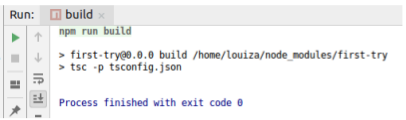
\includegraphics[scale=0.75]{../projet/3.png} 
	\end{tabular}\break

	Lors du débogage(qui peut également être utilisé avec \--\--debug=true ),\\ le \--\--debug=true par défaut consiste également à s'exécuter en mode d'exécution à sec, ce qui empêche l'outil de créer des fichiers.\newline
	En utilisant l'argument \--\--dry-run=false cela pourrait être changé. Par conséquent, cela signifie que les changements se produiront réellement sur le système de fichiers. Si un fichier a été supprimé ou écrasé, il y a un risque de perte de contenu. L'idéal c'est d’être dans un répertoire temporaire séparé lors du débogage des schémas et de désactiver les essais à blanc uniquement lorsque cela est nécessaire.\newline
	
	Nous pouvons également démarrer npm run build \--\-- -w dans un terminal séparé afin de reconstruire automatiquement notre projet schématique lorsqu'un fichier est modifié.\newpage
	
	\textbf{IV. Exemple de collection de schémas}\newline
	
	Il est possible de consulter des exemples  de schémas et de lire le code et les commentaires associés via la commande suivante:\newline
	
	louiza@louiza-Satellite-C660:$\sim$/Documents/M2/LEE/projet/schematics/first-try\$ schematics schematic \--\--name demo\newline
	
	Cela va nous créer une collection de schémas\newline
		
	\begin{tabular}{l}
		CREATE /demo/README.md (639 bytes)\\
		CREATE /demo/package.json (525 bytes)
\\
		CREATE /demo/tsconfig.json (631 bytes)
\\
		CREATE /demo/.gitignore (191 bytes)
\\
		CREATE /demo/src/collection.json (1698 bytes)\\
		CREATE /demo/src/my-full-schematic/index.ts (2455 bytes)
\\
		CREATE /demo/src/my-full-schematic/index\_spec.ts (864 bytes)\\
		CREATE /demo/src/my-full-schematic/schema.json (306 bytes)
\\
		CREATE /demo/src/my-full-schematic/files/test2 (127 bytes)
\\
		CREATE /demo/src/my-full-schematic/files/test\_\_INDEX\_\_ (29 bytes)\\
		CREATE /demo/src/my-other-schematic/index.ts (1346 bytes)
\\
		CREATE /demo/src/my-other-schematic/index\_spec.ts (509 bytes)\\
		CREATE /demo/src/my-schematic/index.ts (1458 bytes)
\\
		CREATE /demo/src/my-schematic/index\_spec.ts (482 bytes)\\
	\end{tabular}\newline

	Si on modifie dans le package.json le chemin de collection.json qui est dans la ligne
	"schematics": "./src/collection.json", par "schematics": "./collection.json" comme le montre la figure ci-dessous
	
	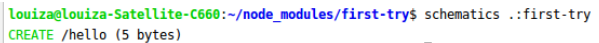
\includegraphics[scale=0.65]{../projet/4.png} 
		
	Notre fichier collection.json prendra les collections de tous les schémas.\\
	
		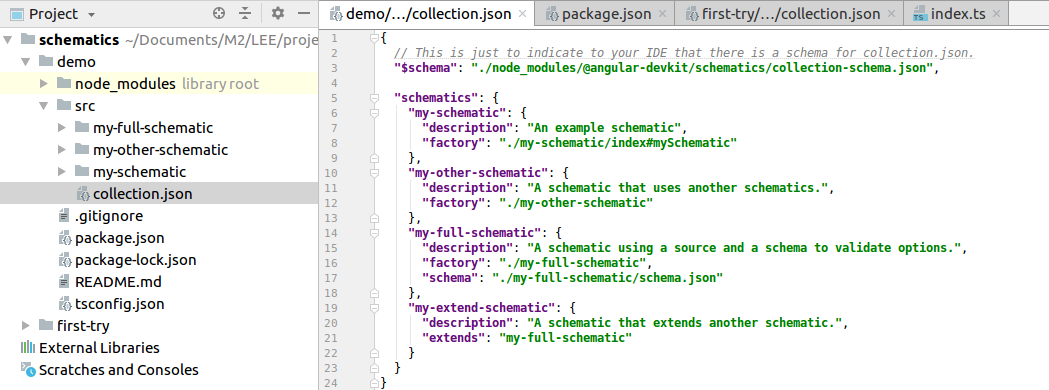
\includegraphics[scale=0.5]{../projet/6.png}  
	
	Cette collection de schémas peut être utilisée avec angular CLI, pour ce faire il faut commencez par créer un projet vide avec la CLI via la commande ng new my-project.
	
	Ensuite, dans le nouveau projet, lier la collection de schémas que nous venons de construire:
\newline	
	npm link \$ PATH\_TO\_SCHEMATIC\_PROJECT\newline 
	
	Il faut remplacer \$PATH\_TO\_SCHEMATIC\_PROJECT par le chemin d'accès à la racine du projet. 
	Une fois le projet de schematics est lié, nous pouvons utiliser ng generate pour appeler les schémas:\newline
	
	ng generate first-try: first-try \\
		 \\
		 \\
		 \\
Lien gitHub: \url{https://github.com/Louizaaaa/angular_schematics.git}  
	
\end{document}\grid
\grid
\grid
\grid
